\documentclass[a4paper]{article}

%%%%%%%% CREATE DOCUMENT STRUCTURE %%%%%%%%
%% Language and font encodings
\usepackage[english]{babel}
\usepackage[utf8x]{inputenc}
\usepackage[T1]{fontenc}
%\usepackage{subfig}

%% Sets page size and margins
\usepackage[a4paper,top=3cm,bottom=2cm,left=2cm,right=2cm,marginparwidth=1.75cm]{geometry}

%% Useful packages
\usepackage{amsmath}
\usepackage{graphicx}
\usepackage[colorinlistoftodos]{todonotes}
\usepackage[colorlinks=true, allcolors=blue]{hyperref}
%\usepackage{caption}
\usepackage[justification=centering]{caption}
\usepackage{subcaption}
\usepackage{sectsty}
\usepackage{float}
\usepackage{titling} 
\usepackage{blindtext}
\usepackage[square,sort,comma,numbers]{natbib}
\usepackage[colorinlistoftodos]{todonotes}
\usepackage{xcolor}
\usepackage{fancyhdr}
\usepackage{lipsum}

%% definitions 
\definecolor{darkgreen}{rgb}{0.0, 0.4, 0.0}

%% Define your personal info here %%%%%%%%%%%%%%%%%%%%%%%
\newcommand\TPid{1}
\newcommand\TPcours{Parallélisme}
\newcommand\TPname{Basics}
\newcommand\Firstname{Joao Filipe}
\newcommand\Familyname{Costa da Quinta}
\newcommand\Email{Joao.Costa@etu.unige.ch}
%%%%%%%%%%%%%%%%%%%%%%%%%%%%%%%%%%%%%%%%%%%%%%%%%%%%%%%

%%%%%%% Page header %%%%%%
\pagestyle{fancy}
\fancyhf{}
\rhead{\TPcours: TP \TPid}
\lhead{\Firstname \; \Familyname}
\rfoot{Page \thepage}


%%%%%%%% DOCUMENT %%%%%%%%
\begin{document}

\section*{Compléxité: Espace}
The goal is to share the same vector bewtween all processus, so the choice of algorithm won't change the results.
Let n be the number of processus and x the space taken by the vector in the system's memory:
\begin{center}
O(n*x) 
\end{center}

\section*{Compléxité: Temps}
Here we'll witness different complexities for each algorithms.
\begin{itemize}
\item[Simple:] Here we have a simple code that uses the command $for$ that iterates the same code for all processus, we have then (n-1) cycles. Let each cycle be of time t, and n processus:  
\begin{center}
O((n-1)*t) , or ->  O(n*t)
\end{center}


\item[Anneau:] It's here we see the interest of parallélisme, we are sending the same amount of information, but sinse we do it in parallel we do lesse cycles. Let time per cycle be t, and n the number of processus:  
\begin{center}
O(2*t + (n-3)/2 * t ), or ->  O((n/2)*t) 
\end{center}

\item[Hypercube:] For this last one, the train of thought is the same, just that we have even more processus sending information:

\begin{itemize} 
\item[cycle 1 -> ] we have 1 processus
\item[cycle 2 -> ] we have 1 processus
\item[cycle 3 -> ] we have 1 processus
\item[ ... ]
\item[cycle n -> ] we have $2^{(n-1)}$ processus
\end{itemize} 

For n processes we will require $log_{2}(n)$ cycles. time t per cycle
\begin{center}
O($log_{2}(n)$*t) 
\end{center}
\end{itemize}
\section*{Résultats}
For the results I used the following code in the batchfile:
\begin{center}
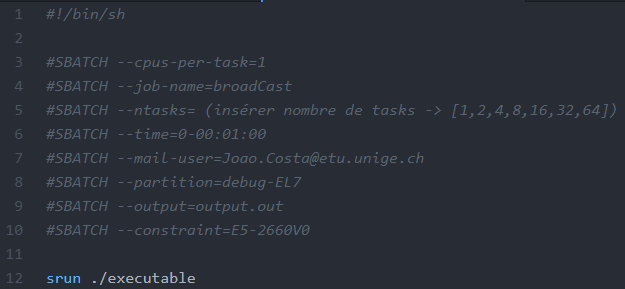
\includegraphics[width=0.7\textwidth]{images/batch.PNG}\\[1cm] 
\end{center}
I had problems to execute this batchfile with nProc = 64, I discussed them with you via email.\\\\\\

For simple, Anneau and Hypercube, I find unexpected results, as Anneau became faster than Hyper as n grew larger. Simple is as expected.

\begin{center}
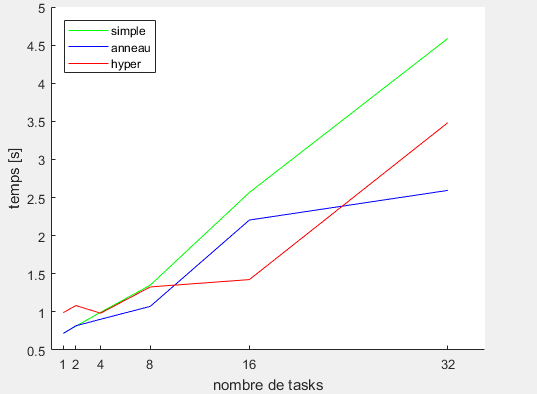
\includegraphics[width=0.7\textwidth]{images/graph.PNG}\\[1cm] 
\end{center}


I don't know why but using the simple BCast command didn't work as intended, it was very slow, I don't know if it was just by chance, but I did try it many times, and I always got the same results

\begin{center}
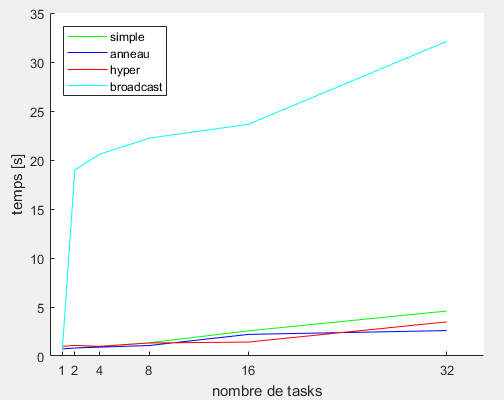
\includegraphics[width=0.7\textwidth]{images/graph2.PNG}\\[1cm] 
\end{center}

I don't want to talk much about the broadcast function results, because they are probably not accurate. However, I theorised that Hypercube algorithm would be less expensive than Anneau, which it is at the beginning, but when we cross the 32 cores mark, Anneau becomes faster, this was theoretically unexpected, but we were told it would be the result.\\
My best guess is that we are not taking full advantage of the structure/architecture, and that we will later on find an algorithm that exploits the same idea but does it in another way, because intuitively Hypercube looks much faster than Anneau.
































\end{document}
